\documentclass{article}
\usepackage[utf8]{inputenc}
\usepackage[dvipsnames]{xcolor}
\usepackage{tikz}
\usetikzlibrary{shapes.geometric, arrows}
\usepackage[skins]{tcolorbox}

\tikzstyle{nnmodel} = [trapezium, draw=black, fill=blue!20, trapezium left angle=120, trapezium right angle=120]
\tikzstyle{textcontainer} = [rectangle]
\tikzstyle{imageframe} = [rectangle]
\tikzstyle{arrow} = [thick, ->, >=stealth, draw=Maroon]
\tikzstyle{nonactivearrow} = [thick, ->, >=stealth, draw=Maroon!30]

\begin{document}

\begin{tikzpicture}[node distance=1.5cm]
    \node (imagelabel) [textcontainer] {Image segment};
    \node (fragimage) [imageframe, right of=imagelabel, xshift=1cm] {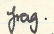
\includegraphics[width=.08\textwidth]{../images/frag.png}};
    \node (m3image) [imageframe , right of=fragimage, xshift=.7cm] {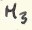
\includegraphics[width=.08\textwidth]{../images/m3.png}};
    \node (azurelabel) [textcontainer, below of=imagelabel, yshift=.5cm] {OCR output};
    \node (frag) [textcontainer, right of=azurelabel, xshift=1cm] {frag.};
    \node (m3) [textcontainer, right of=frag, xshift=.7cm] {H3};
    \node (toothornot) [nnmodel, below of=frag, xshift=1.2cm, yshift=.5cm] {tooth or other?};
    \node (uplow) [nnmodel, below of=toothornot] {upper or lower?};
    \node (mpic) [nnmodel, below of=uplow] {M, P, I or C?};
    \node (mindex) [nnmodel, below of=mpic, xshift=-1.8cm] {1, 2 or 3?};
    \node (pindex) [nnmodel, below of=mpic, xshift=1.8cm] {1, 2, 3 or 4?};
    \node (end) [textcontainer, below of=mpic, yshift=-1.5cm] {frag. m3};

    \draw [arrow, draw=Blue] (frag) -- (toothornot);
    \draw [arrow] (m3) -- (toothornot);
    \draw [arrow] (toothornot) -- node[anchor=east] {tooth} (uplow);
    \draw [arrow] (uplow) -- node[anchor=east] {lower} (mpic);
    \draw [arrow] (mpic) --  node[anchor=east, yshift=0.2cm] {m} (mindex);
    \draw [nonactivearrow] (mpic) -- (pindex);
    \draw [arrow] (mindex) -- node[anchor=east, yshift=-0.2cm] {m3} (end);
    \draw [nonactivearrow] (pindex) -- (end);
    \draw [nonactivearrow] (mindex) -- (end);
    \draw[thick, draw=Blue] (toothornot) -- node[anchor=south] {other} (-1.7,-2) -- (-1.7,-8);
    \draw[->, thick, draw=Blue] (-1.7,-8) -- (2.7,-8);
    \draw[thick, draw=Maroon!30] (mpic) -- (8.5,-5) -- (8.5,-8);
    \draw[->, thick, draw=Maroon!30] (8.5,-8) -- (4.7,-8);
\end{tikzpicture}

 

\end{document}